\documentclass[11pt]{article}
% Author: Kyaw Thi (Eric) Ha — November task explainer for Banking 1B
\usepackage[margin=2.3cm,a4paper]{geometry}
\usepackage[sfdefault]{plex-sans}
\usepackage{plex-mono}
\usepackage{amsmath,booktabs,tabularx,array,colortbl,graphicx,xcolor,enumitem,tikz,caption,titlesec,fancyhdr}
\usepackage{xurl}
\usepackage[colorlinks=true,linkcolor=emerald,urlcolor=emerald,citecolor=emerald]{hyperref}
\usetikzlibrary{positioning,arrows.meta}
\graphicspath{{figs/}}

\definecolor{ink}{HTML}{17211C}
\definecolor{body}{HTML}{2E3833}
\definecolor{muted}{HTML}{5E6862}
\definecolor{panel}{HTML}{ECEEE7}
\definecolor{emerald}{HTML}{16855A}
\definecolor{amber}{HTML}{A97A06}
\color{body}
\newcolumntype{L}{>{\raggedright\arraybackslash}X}
\renewcommand{\arraystretch}{1.25}
\emergencystretch=2em
\setlength{\parskip}{0.55em}\setlength{\parindent}{0pt}
\setlist{itemsep=2pt,topsep=3pt}
\titleformat{\section}{\color{ink}\Large\bfseries}{\color{emerald}\thesection}{0.6em}{}
\titleformat{\subsection}{\color{ink}\large\bfseries}{\color{emerald}\thesubsection}{0.6em}{}
\captionsetup{font={small,color=muted},labelfont={bf,color=ink}}
\pagestyle{fancy}\fancyhf{}\renewcommand{\headrulewidth}{0pt}
\fancyfoot[L]{\color{muted}\scriptsize Banking 1B \textperiodcentered{} Small neural networks \textperiodcentered{} Eric}
\fancyfoot[R]{\color{muted}\scriptsize\thepage}

\newcommand{\note}[2][panel]{\par\noindent\colorbox{#1}{\parbox{\dimexpr\linewidth-2\fboxsep}{\vspace{4pt}#2\vspace{4pt}}}\par}
\newcommand{\eric}{{\color{emerald}\bfseries[Eric]}}

\begin{document}

{\color{emerald}\small\bfseries BREAK THROUGH TECH AI STUDIO \textperiodcentered{} BANKING 1B \textperiodcentered{} NOVEMBER TASK}\\[6pt]
{\raggedright\color{ink}\fontsize{24}{28}\selectfont\bfseries Small Neural Networks for Fraud Detection\par}
\vspace{4pt}
{\large\color{muted} What I built, why each step exists, and what we learned\par}
\vspace{8pt}
{\color{ink}\bfseries Author: Kyaw Thi (Eric) Ha}\ \ {\color{muted}(@KTH-Sys) \textperiodcentered{} November 2026}\\
{\small\color{muted}Notebook: \nolinkurl{notebooks/BTT_Mastercard_Small_Neural_Nets_Eric.ipynb}}

\vspace{6pt}
\note{\eric\ \textbf{Hi team.} My November task was to \textbf{train small neural networks, compare them with our other models, and evaluate them properly}. This document explains every step in plain language, so you can follow it even if you have never trained a network. The notebook has the same structure and all the code; everything here is reproducible from it.}

\section*{The one-minute summary}
\begin{itemize}
\item \textbf{Hidden layers help.} On exactly the same 515-column table, a network with no hidden layers scores like logistic regression (AP 0.438 vs 0.427). Adding hidden layers raises AP to 0.48--0.53.
\item \textbf{Embeddings help the most.} Letting the network learn a small vector for each ID-like value (\texttt{card1}, \texttt{addr1}, email domain, device\ldots) raises AP to \textbf{0.560 on average over 3 seeds}, versus 0.515 without them. The two ranges do not overlap.
\item \textbf{LightGBM is still about 0.07 AP ahead} (0.632), on every metric and in every segment. Blending the network into LightGBM makes it slightly \emph{worse}.
\item \textbf{28\% of fraud is missed by both models} at a 5\% review budget. The next improvement probably needs new information, not a new algorithm.
\item \textbf{Recommendation:} keep LightGBM as the main model; keep the embedding network as our documented deep-learning baseline.
\end{itemize}
All numbers are on the \textbf{validation} period (59,054 transactions). The holdout was never loaded.

% =====================================================================
\section{What question I was answering}
Our baseline notebook showed that boosted trees (LightGBM AP 0.632, XGBoost 0.613) rank fraud far better than logistic regression (0.428). Logistic regression adds up weighted features in a straight line. It cannot learn ``small amount \emph{and} new device \emph{and} unusual email'' unless someone builds that feature by hand. A neural network can learn such combinations itself, so it was the natural next model.

\begin{center}
\begin{tabularx}{\linewidth}{@{}>{\raggedright\arraybackslash\bfseries}p{0.7cm}L>{\raggedright\arraybackslash}p{5.3cm}@{}}
\toprule
& \textbf{Question} & \textbf{My guess before running} \\
\midrule
Q1 & Does a small network beat logistic regression on the \emph{same} inputs? & Yes \\
Q2 & Does a bigger network help? & A little, then it stops \\
Q3 & Does giving fraud rows extra weight help? & Ranking barely changes \\
Q4 & Do embeddings for high-cardinality categories help? & Yes \\
Q5 & How close does the best network get to LightGBM? Is it stable? & Below LightGBM, stable \\
Q6 & Does blending it with LightGBM add anything? & Maybe a little \\
Q7 & Where is it weak, and are its scores real probabilities? & Weak where history is thin \\
\bottomrule
\end{tabularx}
\end{center}

% =====================================================================
\section{The data I used}
I did \textbf{not} redo any preprocessing. I loaded the tables our feature-engineering notebook already saved, because their rules (medians, scalers, encodings) were fitted on the training period only. Redoing them in a new place is an easy way to leak future information.

\begin{center}
\begin{tabularx}{\linewidth}{@{}>{\raggedright\arraybackslash\bfseries}p{3.6cm}L@{}}
\toprule
Split & Train: 472,432 transactions (first 80\% in time). Validation: the next 59,054. Holdout: the last 59,054 (\textbf{not loaded}). \\
Neural-net table (515 cols) & Skewed columns log-transformed, extremes clipped, gaps filled with the training median, everything standardized (mean 0, standard deviation 1), plus missing-value flags and one-hot columns for categories with at most 10 values. \\
Tree table (537 cols) & Categories and missing values kept as they are. Used for LightGBM and as the source of the embedding columns. \\
\bottomrule
\end{tabularx}
\end{center}

\textbf{Sanity checks I run first:} labels line up row by row with the features, no forbidden columns (\texttt{isFraud}, \texttt{TransactionID}, \texttt{TransactionDT}), and \textbf{no missing or infinite values} in the numeric table, because a single missing value makes a network output ``not a number'' for everything.

\textbf{Check that I matched the team:} my logistic regression gives AP 0.4273 (team 0.4276), and my LightGBM gives exactly 0.6315 (team 0.6315). So my comparison uses the same data as everyone else's.

% =====================================================================
\section{How a small neural network works}
\textbf{Start with logistic regression.} It computes one weighted sum of the inputs and squashes it into a number between 0 and 1:
\[
p(\text{fraud}) = \sigma\!\left(b + w_1x_1 + \dots + w_px_p\right), \qquad \sigma(z) = \frac{1}{1+e^{-z}}.
\]
\textbf{A neural network adds hidden layers in between.} Each hidden \emph{neuron} computes its own weighted sum and then applies \textbf{ReLU}: keep the value if it is positive, otherwise output 0. That small bend is what allows stacked layers to build ``if this \emph{and} that'' rules. The next layer combines those outputs again, and the last neuron gives the fraud score.

\begin{center}
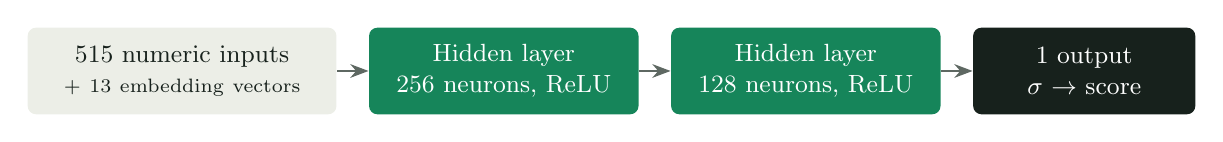
\begin{tikzpicture}[node distance=0.4cm, every node/.style={font=\small, rounded corners=3pt, inner sep=6pt, align=center, minimum height=1.1cm}]
  \node[fill=panel,text=ink,text width=3.5cm] (in) {515 numeric inputs\\{\scriptsize + 13 embedding vectors}};
  \node[fill=emerald,text=white,text width=3.0cm,right=of in] (h1) {Hidden layer\\\mbox{256 neurons}, ReLU};
  \node[fill=emerald,text=white,text width=3.0cm,right=of h1] (h2) {Hidden layer\\\mbox{128 neurons}, ReLU};
  \node[fill=ink,text=white,text width=2.4cm,right=of h2] (out) {1 output\\$\sigma$ $\rightarrow$ score};
  \draw[-{Stealth},muted,thick] (in)--(h1); \draw[-{Stealth},muted,thick] (h1)--(h2); \draw[-{Stealth},muted,thick] (h2)--(out);
\end{tikzpicture}
\end{center}

A network with \textbf{zero} hidden layers \emph{is} logistic regression. That is why I trained one as a control: if the real networks beat it, the gain must come from the hidden layers, not from my training code.

\subsection{How it learns}
\begin{center}
\begin{tabularx}{\linewidth}{@{}>{\raggedright\arraybackslash\bfseries}p{3.6cm}L>{\raggedright\arraybackslash}p{3.3cm}@{}}
\toprule
Term & Meaning & My setting \\
\midrule
Loss & A penalty that is large when a fraud gets a low score or a legitimate payment gets a high score. Training makes it small. & Binary cross-entropy \\
Mini-batch & Look at a small group of rows, adjust the weights a little, then take the next group. & 2,048 rows \\
Epoch & One full pass over all training rows. & $\approx$231 mini-batches \\
Optimizer & The rule for how big each adjustment is. & Adam, learning rate 0.001 \\
Batch normalization & Re-centres each layer's outputs; faster, steadier training. & After every hidden layer \\
Dropout & Randomly switches off some neurons while training, so the network cannot memorize one path. & 0.1--0.3 \\
Weight decay & A tiny penalty on large weights (like \texttt{C} in logistic regression). & $10^{-5}$ \\
Early stopping & Score validation after every epoch, keep the best epoch, stop after 4 epochs without improvement. & Patience 4, max 25 \\
\bottomrule
\end{tabularx}
\end{center}

\subsection{Embeddings, in one paragraph}
Columns such as \texttt{card1} (12,730 values) or \texttt{addr1} are \textbf{ID codes stored as numbers}. In the numeric table they are standardized like dollar amounts, which tells the network that card group 9500 is ``bigger'' than 7919. That is meaningless. An \textbf{embedding} gives every common value its own short vector (up to 16 numbers), learned during training, so values with similar fraud behaviour end up close together. I used embeddings for 13 columns: \texttt{card1}, \texttt{card2}, \texttt{card3}, \texttt{card5}, \texttt{addr1}, \texttt{addr2}, both email domains, email provider, device family, browser (\texttt{id\_31}), OS (\texttt{id\_30}) and screen size (\texttt{id\_33}). Values seen fewer than 20 times in training share one ``rare/unseen'' slot. A missing value is its own category, because our EDA showed that missingness itself carries fraud signal.

% =====================================================================
\section{How we measure}
I reused the team's \texttt{evaluate()} function \textbf{unchanged}, so my numbers sit in the same table as everyone else's.
\begin{itemize}
\item \textbf{Average precision (AP)} --- the main score. It summarizes precision across every catch rate. Random guessing scores the fraud rate, about \textbf{0.031}.
\item \textbf{Recall at 1\% FPR} --- out of 100 frauds, how many we catch if we may flag at most 1\% of legitimate customers.
\item \textbf{TFPR} (the advisor's ratio) --- legitimate alerts per fraud caught. ``0.5'' means one false alert for every two frauds caught.
\item \textbf{Top-5\% capture} --- the share of fraud found if analysts review only the riskiest 5\% of transactions.
\end{itemize}

\note{\textbf{One caveat applies to every number below.} Early stopping looks at validation to decide when to stop, and I also use validation to compare models. That makes validation scores slightly optimistic, exactly like the trees' early stopping in the baseline notebook. The untouched holdout will give the honest number for the final model.}

% =====================================================================
\section{Experiments and results}
I changed \textbf{one thing at a time}; everything else stayed fixed (same rows, inputs, optimizer and stopping rule, seed 0).

\begin{figure}[h]
\centering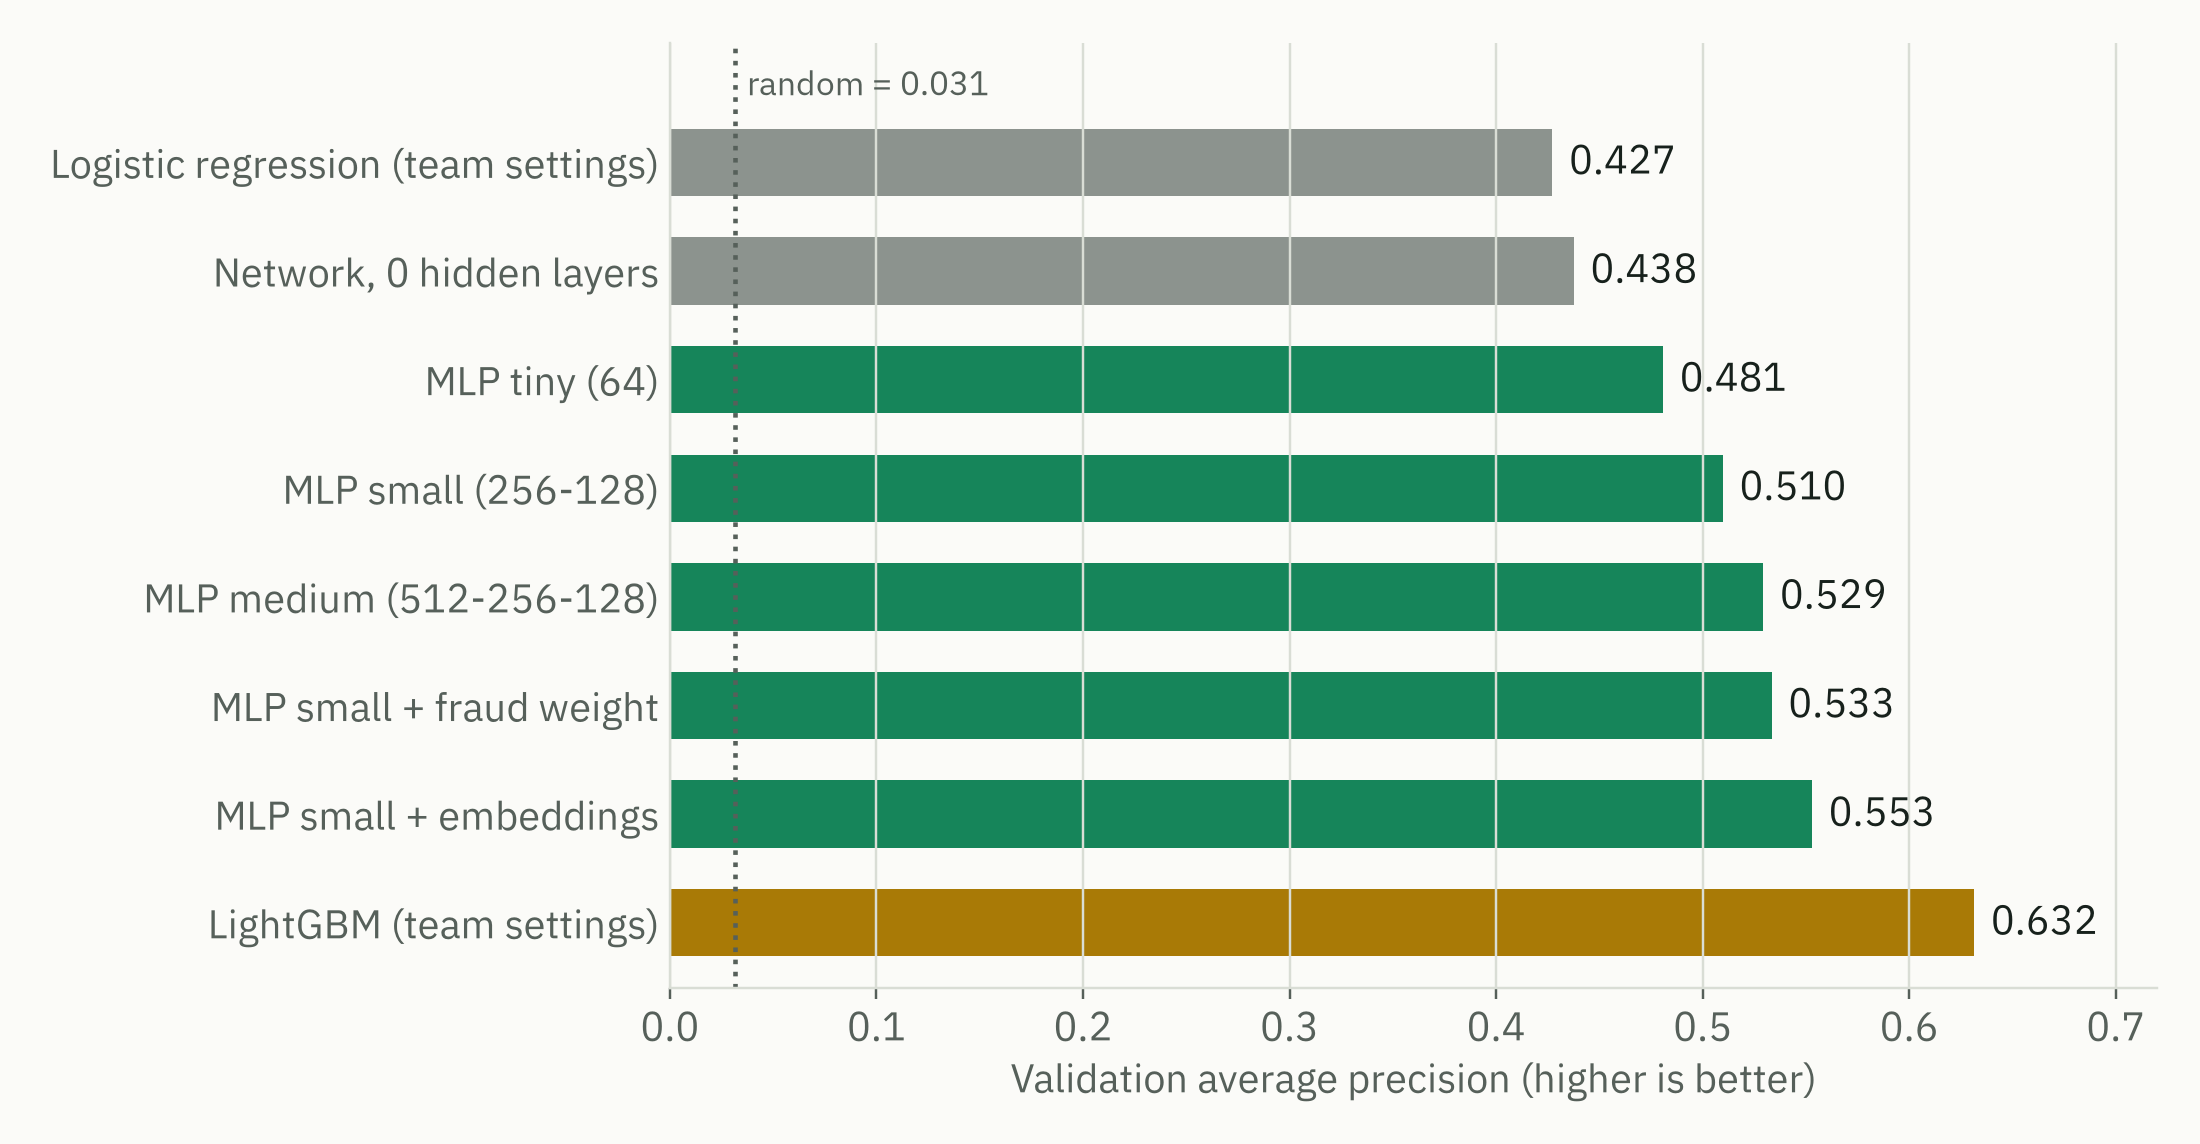
\includegraphics[width=0.86\linewidth]{fig_ap_bars.png}
\caption{Validation AP for every model (seed 0). Gray: linear models. Emerald: neural networks. Amber: LightGBM trained with the team's settings.}
\end{figure}

\begin{center}
\small
\begin{tabularx}{\linewidth}{@{}L rrrrr@{}}
\toprule
\textbf{Model} & \textbf{Weights} & \textbf{AP} & \textbf{Recall @1\% FPR} & \textbf{TFPR @50\%} & \textbf{Top-5\%} \\
\midrule
Logistic regression (team settings) & 516 & 0.427 & 37.6\% & 1.99 & 50.8\% \\
Network, 0 hidden layers & 516 & 0.438 & 38.0\% & 2.02 & 50.7\% \\
MLP tiny (64) & 33k & 0.481 & 41.1\% & 1.57 & 54.5\% \\
MLP small (256--128) & 166k & 0.510 & 44.6\% & 1.10 & 57.8\% \\
MLP medium (512--256--128) & 430k & 0.529 & 47.9\% & 0.79 & 60.1\% \\
MLP small + fraud weight 5.2$\times$ & 166k & 0.533 & 46.4\% & 0.85 & 58.9\% \\
\rowcolor{panel} MLP small + embeddings & 266k & \textbf{0.553} & \textbf{49.9\%} & \textbf{0.63} & \textbf{60.6\%} \\
LightGBM (team settings) & -- & 0.632 & 56.4\% & 0.34 & 68.4\% \\
\bottomrule
\end{tabularx}
\end{center}

\subsection*{Q1 --- Do hidden layers help? \textcolor{emerald}{Yes.}}
The zero-hidden-layer network lands next to logistic regression, so my training loop is not secretly better on its own. A single hidden layer of 64 neurons jumps to 0.481. The inputs are identical, so the gain comes from learning combinations of features. At a 1\% false-alarm budget, the small network catches about 45 of every 100 frauds versus 38 for logistic regression.

\subsection*{Q2 --- Does a bigger network help? \textcolor{amber}{A little, less each time.}}
33k $\rightarrow$ 166k weights adds +0.029 AP; 166k $\rightarrow$ 430k adds +0.019 but takes about three times longer to train (1.9 vs 0.6 minutes). Single seed, so ``likely, not proven''.

\subsection*{Q3 --- Does weighting fraud rows help? \textcolor{amber}{Promising, not confirmed.}}
My guess was wrong: weighting fraud rows 5.2$\times$ raised AP from 0.510 to 0.533. That is several times the seed noise I measured for the plain network ($\pm$0.005), but I only ran one seed of the weighted model. A likely reason: with early stopping the network only gets 10--20 passes over the data, and the extra weight makes it spend more of them on fraud. The cost is that its scores are inflated (Section~\ref{sec:cal}).

\subsection*{Q4 --- Do embeddings help? \textcolor{emerald}{Yes, the largest gain.}}
AP 0.510 $\rightarrow$ 0.553 (seed 0), recall at 1\% FPR 44.6\% $\rightarrow$ 49.9\%, legitimate alerts per fraud at 50\% detection 1.10 $\rightarrow$ 0.63, with about the same training time.

\subsection{Over-fitting: what the learning curves show}
\begin{figure}[h]
\centering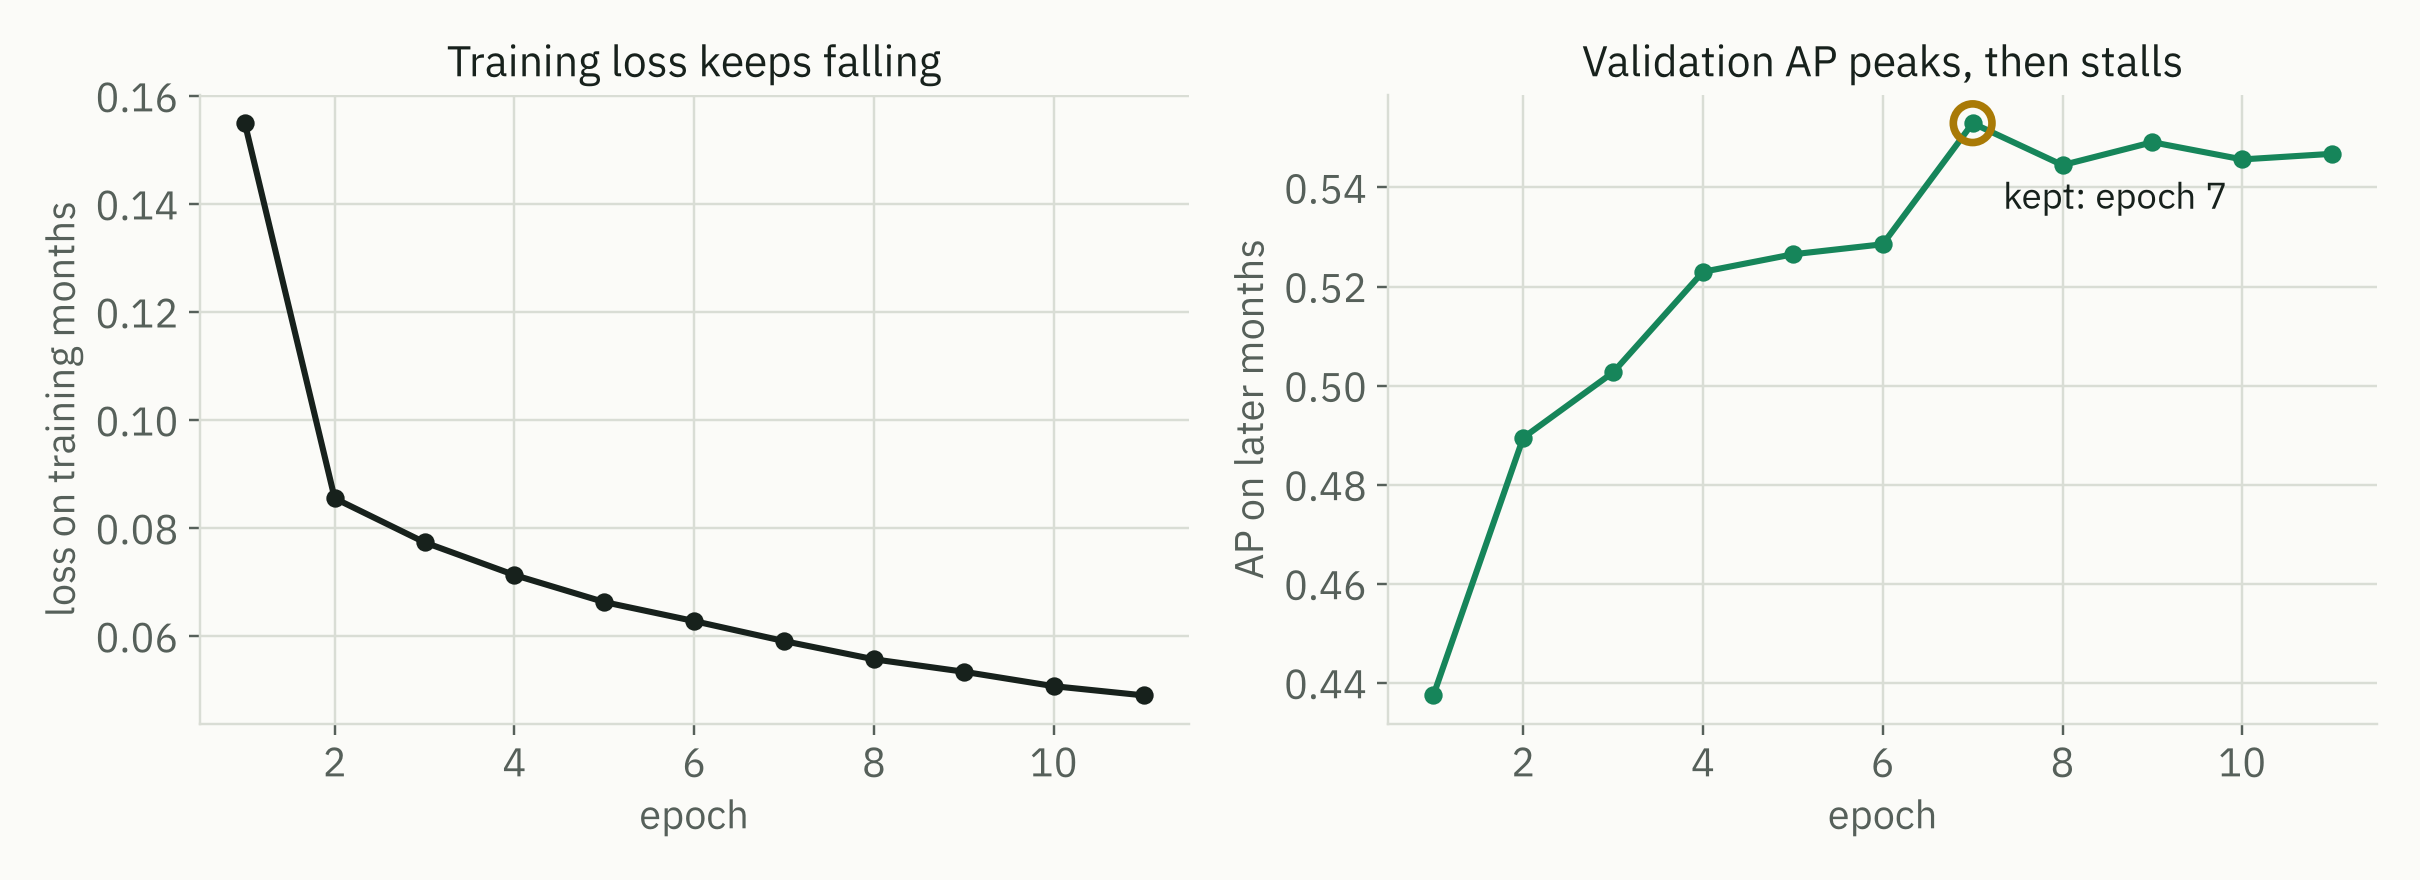
\includegraphics[width=0.92\linewidth]{fig_learning_curve.png}
\caption{The embedding network, epoch by epoch. Training loss keeps falling; validation AP peaks at epoch 7 and then stalls. Early stopping keeps the circled epoch.}
\end{figure}
Every network shows this pattern. When the training score keeps improving but the validation score stops, the network has started learning patterns that only exist in the training months: that is \textbf{over-fitting}. The embedding model peaks earliest (epoch 7), because embeddings learn quickly and then start memorizing category-specific quirks.

\subsection{Q5a --- Is the gain real? Three random seeds}
A network starts from random weights and sees mini-batches in random order, so two runs can differ by chance. I retrained the plain and the embedding network with seeds 0, 1 and 2.
\begin{figure}[h]
\centering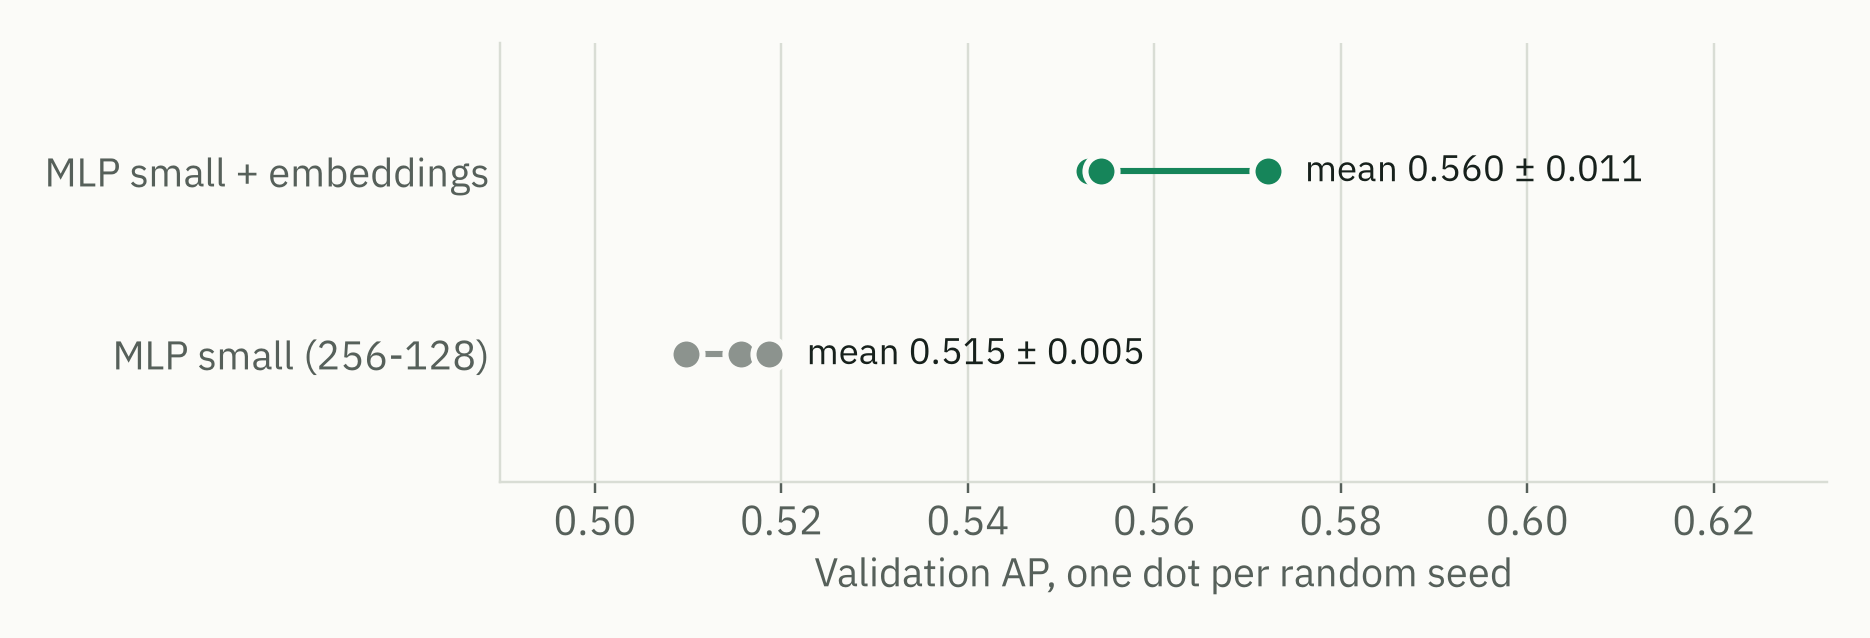
\includegraphics[width=0.78\linewidth]{fig_seeds.png}
\caption{One dot per seed. The worst embedding run (0.553) beats the best plain run (0.519).}
\end{figure}

\begin{center}
\begin{tabular}{@{}lrrrr@{}}
\toprule
\textbf{Model} & \textbf{Seed 0} & \textbf{Seed 1} & \textbf{Seed 2} & \textbf{Mean $\pm$ std} \\
\midrule
MLP small & 0.510 & 0.516 & 0.519 & 0.515 $\pm$ 0.005 \\
MLP small + embeddings & 0.553 & 0.572 & 0.554 & \textbf{0.560 $\pm$ 0.011} \\
\bottomrule
\end{tabular}
\end{center}
The +0.045 gain is 4--10 times the seed spread, so I am confident it is real on this validation period. The embedding model wobbles more, because rare categories get few updates and depend more on the random start.

% =====================================================================
\section{Comparison with LightGBM}
\subsection{Q5b --- Head to head}
\begin{figure}[h]
\centering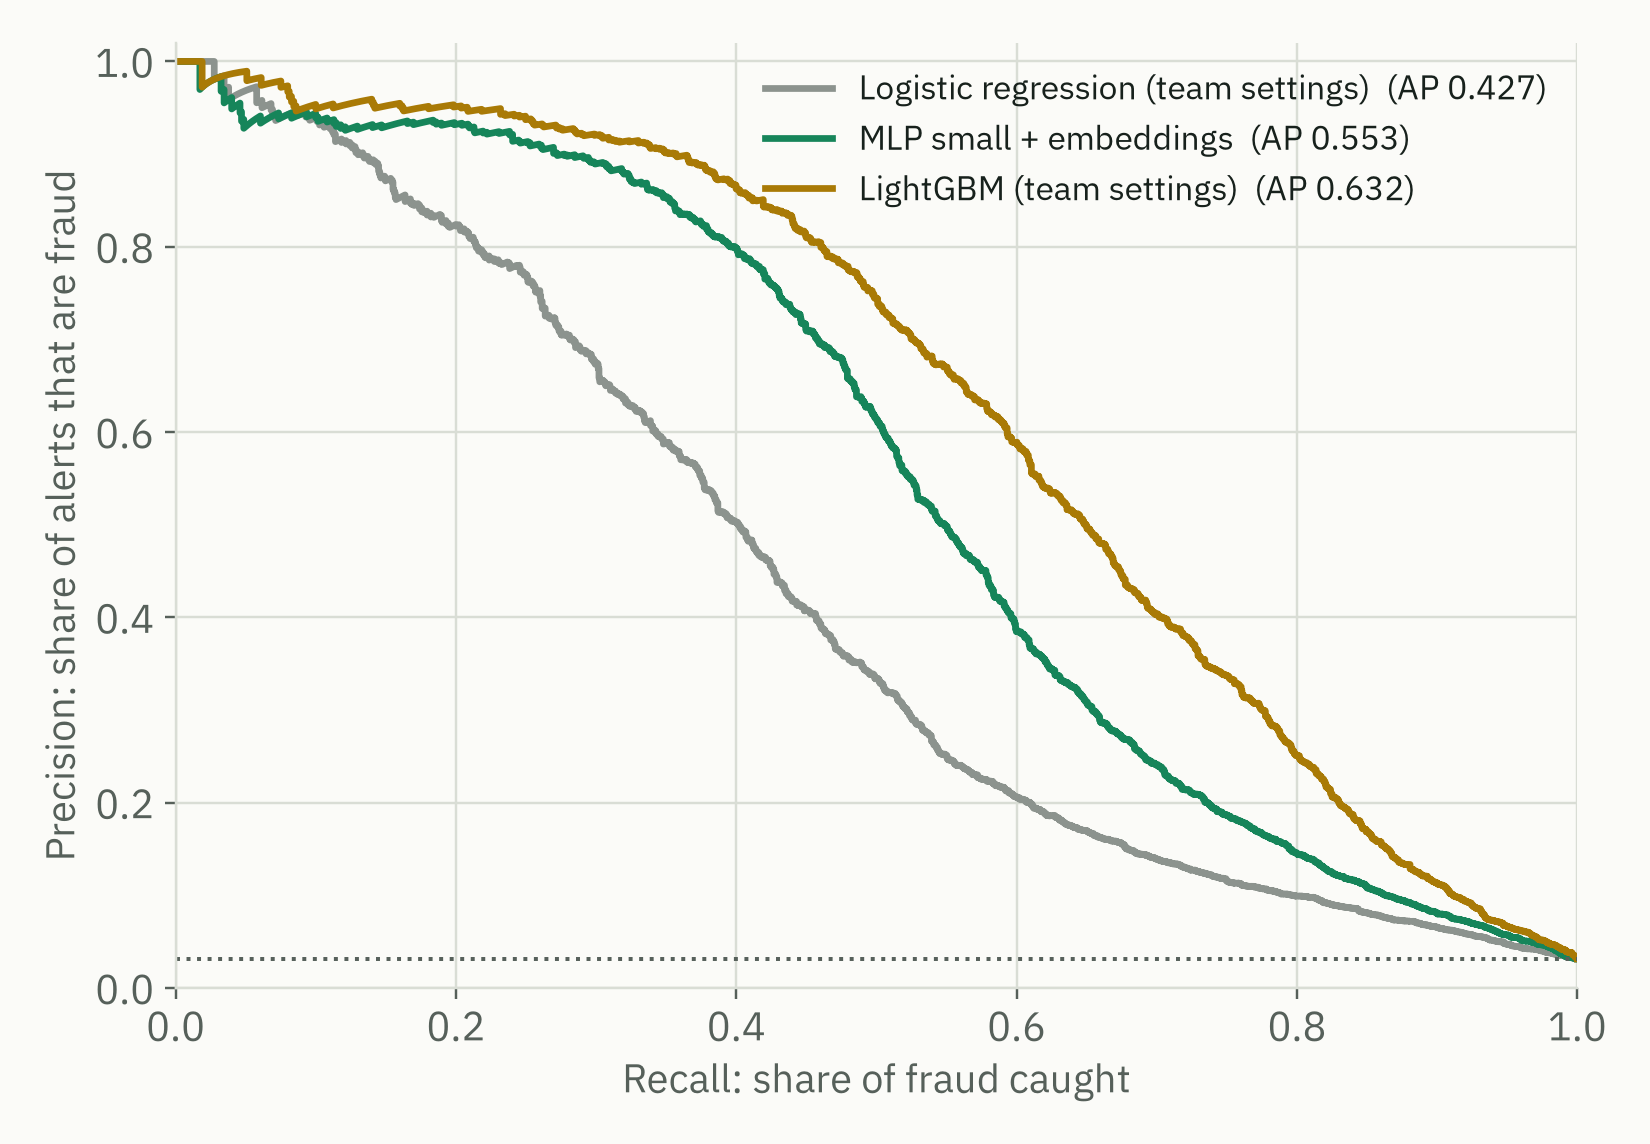
\includegraphics[width=0.62\linewidth]{fig_pr_curves.png}
\caption{Precision--recall curves on validation. Higher and further right is better.}
\end{figure}

\begin{center}
\begin{tabular}{@{}lrrr@{}}
\toprule
\textbf{Legitimate alerts per fraud caught (TFPR)} & \textbf{Logistic regr.} & \textbf{Best network} & \textbf{LightGBM} \\
\midrule
To catch 50\% of fraud & 1.99 & 0.63 & \textbf{0.34} \\
To catch 70\% & 6.19 & 3.15 & \textbf{1.48} \\
To catch 80\% & 9.08 & 5.88 & \textbf{2.98} \\
To catch 90\% & 14.34 & 11.34 & \textbf{7.81} \\
\bottomrule
\end{tabular}
\end{center}
The network closes about 60\% of the gap between logistic regression and LightGBM. \textbf{Only LightGBM stays under the advisor's rough 10:1 ratio at 90\% detection.} Training time is not the issue (0.6 vs 2.6 minutes). Trees handle missing values, extreme values and sharp cut-offs natively, while the network only sees the median-filled, standardized table, where some of that information is smoothed away. This matches what most tabular-data comparisons report.

\subsection{Q6 --- Does blending help? \textcolor{amber}{No.}}
I blended by \emph{rank} (convert each model's scores to 0--1 ranks, then take a weighted average) and judged it with the team's time-block bootstrap (resample 100 consecutive blocks of validation time, 300 times).

\begin{center}
\begin{tabular}{@{}lrrr@{}}
\toprule
\textbf{Weight on the network} & \textbf{AP} & \textbf{Change vs LightGBM} & \textbf{95\% interval} \\
\midrule
10\% & 0.628 & $-$0.004 & $-$0.007 to $-$0.0001 \\
20\% & 0.623 & $-$0.008 & $-$0.014 to $-$0.003 \\
30\% & 0.619 & $-$0.013 & $-$0.020 to $-$0.006 \\
50\% & 0.608 & $-$0.023 & $-$0.033 to $-$0.015 \\
\bottomrule
\end{tabular}
\end{center}
Every interval stays below zero. The reason is visible when we count \textbf{which frauds each model catches} in its top 5\%: both catch 1,061 (57\%); only LightGBM 205 (11\%); only the network 60 (3\%); \textbf{both miss 525 (28\%)}. The network mostly finds frauds LightGBM already finds, so it has little to add.

% =====================================================================
\section{Q7 --- Segments and calibration}\label{sec:cal}
\begin{center}
\small
\begin{tabular}{@{}lrrrrr@{}}
\toprule
\textbf{Segment} & \textbf{Rows} & \textbf{Fraud rate} & \textbf{Logistic} & \textbf{Network} & \textbf{LightGBM} \\
\midrule
Product C & 5,628 & 11.8\% & 0.731 & 0.756 & 0.804 \\
Product H & 1,561 & 5.4\% & 0.464 & 0.528 & 0.625 \\
Product R & 2,558 & 4.7\% & 0.724 & 0.814 & 0.858 \\
Product S & 1,064 & 6.6\% & 0.324 & 0.582 & 0.668 \\
Product W & 48,243 & 1.9\% & 0.116 & 0.356 & 0.461 \\
Identity present & 10,360 & 8.9\% & 0.684 & 0.734 & 0.787 \\
Identity missing & 48,694 & 1.9\% & 0.118 & 0.358 & 0.462 \\
Address missing & 5,486 & 12.1\% & 0.738 & 0.758 & 0.806 \\
\bottomrule
\end{tabular}
\end{center}
\textbf{Read across a row, not down a column}: a segment with more fraud has a higher AP even for a random model. The network trails LightGBM everywhere. The gap is smallest ($\approx$0.05) where fraud is concentrated and identity data exists, and largest ($\approx$0.10) on product W and identity-missing transactions, the same weak spot the team found for XGBoost. On product W the network triples logistic regression's AP.

\begin{minipage}[t]{0.47\linewidth}\vspace{0pt}
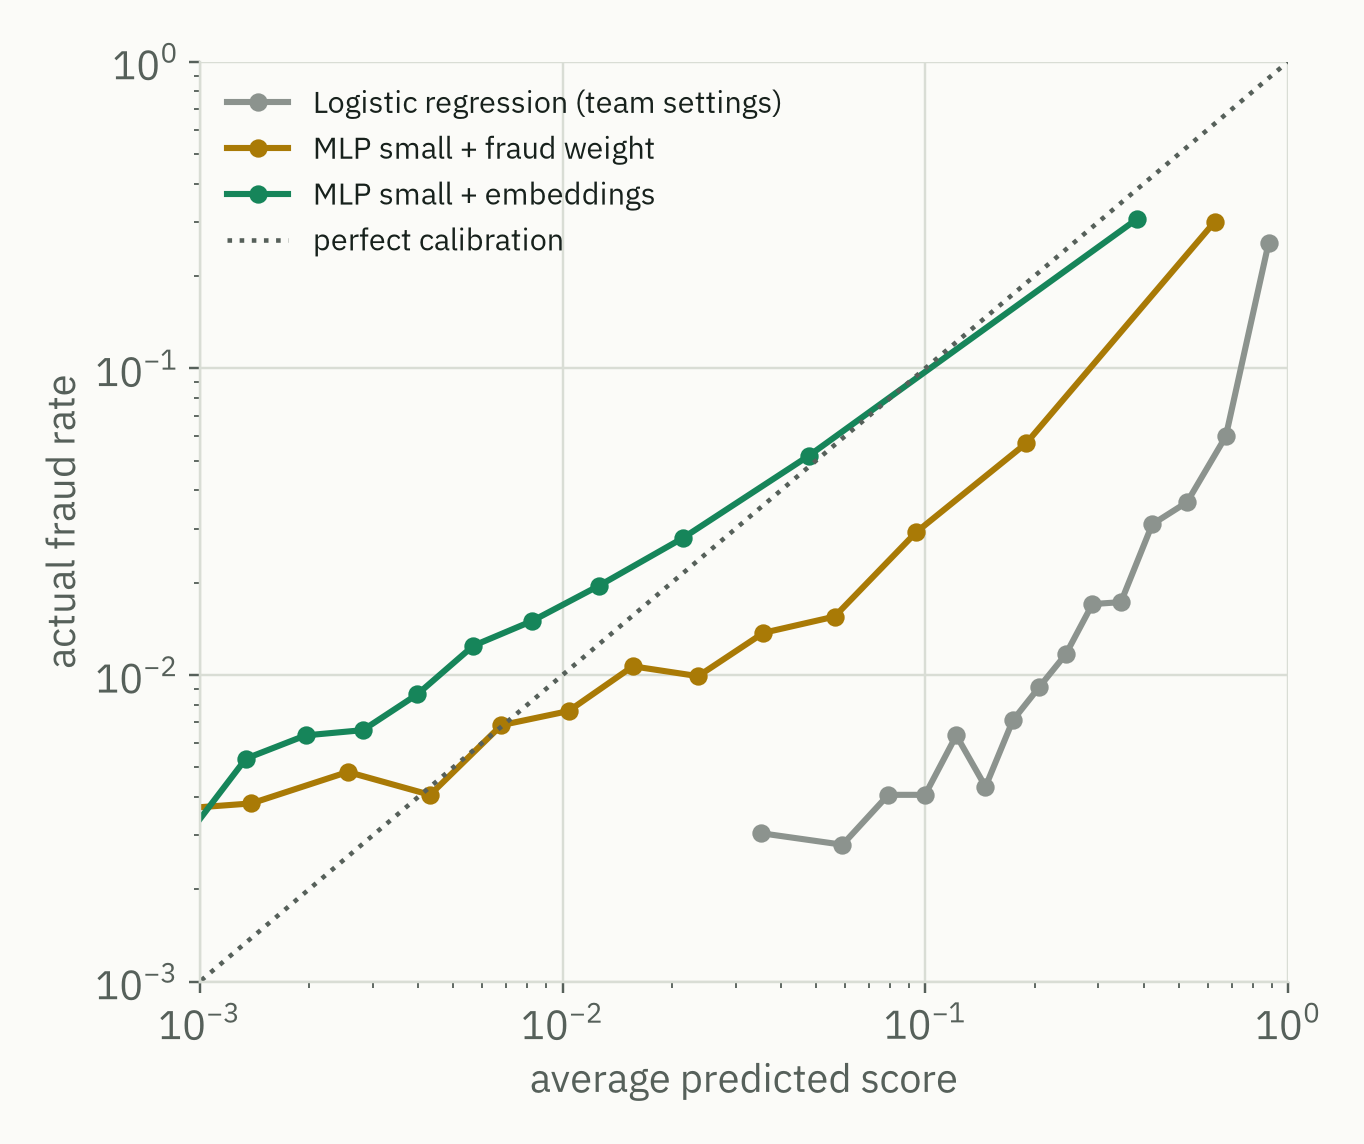
\includegraphics[width=\linewidth]{fig_calibration.png}
\end{minipage}\hfill
\begin{minipage}[t]{0.5\linewidth}\vspace{4pt}
\textbf{Calibration} asks: if the model says 0.30, are about 30\% of those transactions really fraud?
\begin{itemize}
\item The \textbf{unweighted network} averages 0.033 against a true fraud rate of 0.031, so its scores can be read as probabilities (Brier score 0.020).
\item \textbf{Weighting inflates scores}: the weighted network over-states risk about 2$\times$, and balanced logistic regression about 9$\times$ (average score 0.287).
\item Ranking is unaffected, so for a review budget this is fine. To show analysts a ``probability of fraud'', use an unweighted model or recalibrate.
\end{itemize}
\end{minipage}

% =====================================================================
\section{Things I learned that will save you time}
\begin{itemize}
\item \textbf{PyTorch and LightGBM in one process can freeze on macOS.} Each ships its own OpenMP threading library. My first run hung at 0\% CPU inside LightGBM. The notebook now trains LightGBM in a separate Python process.
\item \textbf{pandas 3 keeps missing values when converting to text.} \texttt{astype(str)} no longer turns NaN into the string \texttt{"nan"}, so missing addresses were silently grouped with rare values. I now label them \texttt{\_\_MISSING\_\_} explicitly.
\item \textbf{Save predictions, not just scores.} Every model saves its validation predictions, so the whole notebook re-runs in about 30 seconds and later analyses (blends, segments, overlap) need no retraining.
\item \textbf{Always train a ``zero-hidden-layer'' control.} It separates ``hidden layers help'' from ``my training loop is different''.
\end{itemize}

% =====================================================================
\section{Limitations and next steps}
\textbf{Limitations.} Validation is used for early stopping and model choice, so it is optimistic. Most comparisons are one seed; only two models have three. Nothing is tuned (learning rate, dropout, embedding size are sensible defaults), and the trees are not tuned either. There is only one validation period of about three weeks, and fraud patterns drift.

\textbf{Proposed next steps.}
\begin{enumerate}
\item Combine what helped (embeddings + fraud weighting, maybe the medium size), over 3 seeds.
\item Add embeddings for the team's account keys, so the network sees account identity directly.
\item Study the 525 frauds both models miss (likely concentrated in product W and identity-missing rows) and plan features for them as a team.
\item If time allows, a small sequence model (GRU) over each account's recent transactions. Trees cannot do this easily.
\item When the team freezes the final model, score the holdout \textbf{once}.
\end{enumerate}

\section*{How to reproduce}
\begin{enumerate}
\item Download the data (\texttt{bash} \nolinkurl{scripts/download_data.sh}) and run \nolinkurl{BTT_Mastercard_Feature_Engineering_Final.ipynb}; it writes \nolinkurl{outputs/feature_engineering/fe_final_v1/}.
\item Open \nolinkurl{notebooks/BTT_Mastercard_Small_Neural_Nets_Eric.ipynb} and run all cells. With \texttt{RETRAIN = False}, saved predictions are reused; set it to \texttt{True} to retrain everything (about 15 minutes on a laptop CPU).
\item Results, figures and a reproducibility record (\texttt{record.json}) are written to \nolinkurl{outputs/feature_engineering/fe_final_v1/neural_nets/eric_v1/}.
\end{enumerate}

\end{document}
